\documentclass[conference]{IEEEtran}
\usepackage{cite}
\usepackage[portuges,brazil]{babel}
\usepackage{amsmath,amssymb,amsfonts}
\usepackage{siunitx}
\usepackage{algorithmic}
\usepackage{graphicx}
\usepackage{textcomp}
\usepackage{hyperref}
\usepackage{listings}
\usepackage[toc,page]{appendix}
\usepackage[utf8]{inputenc}

\def\BibTeX{{\rm B\kern-.05em{\sc i\kern-.025em b}\kern-.08em
    T\kern-.1667em\lower.7ex\hbox{E}\kern-.125emX}}

\begin{document}

\title{Projeto 2: Aplicação de Técnicas de limiarização\\
\large .\\
\large MC920 - Introduçãao ao Processamento Digital de Imagem (MC920 / MO443) 2S2019\\
\large Professor: Hélio Pedrini}

\newcommand{\email}[1]{\href{mailto:#1}{#1}}

\author{
    \IEEEauthorblockN{Giovani Nascimento Pereira}
    \IEEEauthorblockA{
    \email{giovani.x.pereira@gmail.com} \\
    168609
    }
}

\maketitle

\section{Definição do problema}

Métodos de limiarização de imagens, são métodos aplicados para separar o conjunto de pixels de uma imagem em 2 grupos, stribuindo níveis de limítrofes (0 e 255) a cada um dos conjuntos.

Tais métodos podem ser utilizados para extrair detalhes de uma imagem, bem como separar o fundo da informação mais a frente, bem como outras aplicações.

\subsection{Objetivo}

O objetivo deste projeto é implementar e comparar diversos métodos de limiarização, aplicando à imagens em escalas de cinza (no formato .pgm), apresentando os resultados na forma das imagens obtidas e dos histogramas das mesmas, a fim de comparar as distribuições resultantes de níveis de cinza.

\subsection{Execução do projeto}

O projeto pode ser executado utilizando o comando:

\begin{lstlisting}[language=bash]
$ python3 main.py [imagem] [flags]
\end{lstlisting}

Onde o parâmetro \textit{flag} define qual método será executado.

Os métodos implementados podem ser observados a seguir:

\begin{itemize}
    \item \textit{-g} Global
    \item \textit{-b} Burkes
    \item \textit{-n} Niblack
    \item \textit{-c} Contraste
    \item \textit{-avg} Media
    \item \textit{-med} Mediana
    \item \textit{-sp} Sauvola-Pietaksinen
\end{itemize}

Então, por exemplo, caso queira executar o programa para uma imagem na raíz do projeto com o método de Bernsen, ele pode ser executado como:

\begin{lstlisting}[language=bash]
$ python3 main.py image.pgm -b
\end{lstlisting}

Também é possível consultar a documentação do programa usando o comando:

\begin{lstlisting}[language=bash]
$ python3 main.py --help
\end{lstlisting}

E mais de uma flag pode ser usada a cada execução.

\subsection{Limitações do projeto}

Para abrir as imagens, foi utilizada a biblioteca \textit{imageio}. Isso não se mostrou uma boa escolha, pois a biblioteca foi apenas capaz de reconhecer imagens em formato pgmb, ou seja, o formato binário de imagens pgm.

Existe também o formato pgma, que é uma mesma representação mas em ASCII, ou seja, em formato de texto.

É importante ressaltar que ambos os formatos (pgmb e pgma) tem a mesma extensão de arquivo (.pgm), mas podem ser facilmente reconhecidos abrindo com um editor de texto os arquivos, pgma pode ser observados na forma de matrizes em texto puro, já os pgmb não.

Para computar os resultados, o tamanho padrão da janela utilizado, se não especificado, foi de 7x7 pixels da imagem.

\section{Métodos de Limiarização}

\subsection{Global}

    O método de limiarização global é o mais simples de ser implementado, e basta ter um limiar $T$ para dividir os pixels em dois conjuntos, $f(x,y) >= T$ e $f(x, y) < T$, atribuindo 255 e 0 aos pixels respectivamente.

    Esse método nos dá imagens binárias as quais a qualidade visual e o efeito de limiarização depende muito do limiar $T$ escolhido. Um exemplo pode ser observado na imagem \ref{fig:global}

    \begin{figure}[ht]
        \centering
        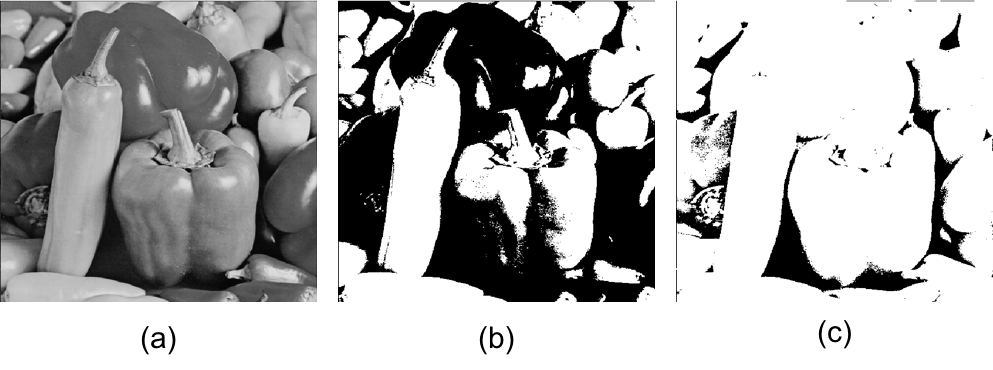
\includegraphics[width=\linewidth]{global.png}
        \caption{Imagens geradas através da aplicação do método de limiarização global para o \textit{peppers.png}. a, original. b limiarizada com $T=128$, c limiarizada com $T=50$.}
        \label{fig:gobal}
    \end{figure}

    De maneira geral, os resultados deste método não são muito bons se comparados aos demais estudados neste projeto.

    Podemos observar na imagem \ref{fig:histo-comp} a distribuição dos níveis de cinza das imagens \ref{fig:global}. Isso mostra os resultados do processo de limiarização.

    \begin{figure}[ht]
        \centering
        \includegraphics[width=\linewidth]{histogram-comparison.png}
        \caption{Histogramas obtidos pelo processamento de limiarização global. (a) é da imagem original e (b) da imagem obtida após a aplicação do método de limiarização global.}
        \label{fig:histo-comp}
    \end{figure}

\subsection{Bersen}

    No método de Bersen, para cada pixel $(x,y)$ da imagem, é calculado um limiar $T$ conforme a \ref{bersen}, onde $z_{min}$ e $z_{max}$ são os o mínimo e máximo local numa vizinhança de dimensão $n*n$ da imagem em relação ao pixel $(x,y)$.

    \begin{equation}
      T(x,y) = \dfrac{z_{min} + z_{max}}{2}
    \label{bersen}
    \end{equation}

    O resultado da aplicação deste método é uma imagem binária mas com um efeito interessante - surgem pontilhados nas áreas que tendem a ser homogêneas da imagem. Se for uma região escura, surgem pontos brancos e vice-versa.
    E quão maior for a vizinhança $n$ mais espaçados são esses pontilhados.
    Esse efeito pode ser observado na figura \ref{fig:bersen}.

    \begin{figure}[ht]
        \centering
        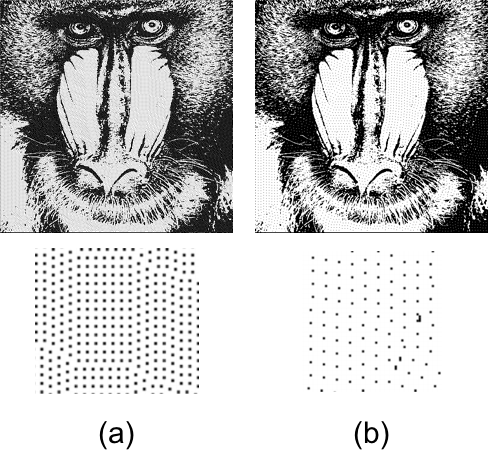
\includegraphics[width=\linewidth]{bersen.png}
        \caption{Imagens geradas através da aplicação do método de limiarização de Burkes para o \textit{baboon.png}, para $n = 4$ e $n = 10$, respectivamente a e b, com um corte em zoom da mesma área das duas imagens para comparação.}
        \label{fig:bersen}
    \end{figure}

\subsection{Contraste}

    O método do contraste consiste em simplesmente tomar o mínimo e máximo local, dentro de uma janela, e segmentar os pixels baseados em qual dos limites ele está mais próximo.

    É possível observar os resultados da aplicação deste método na figura \ref{fig:contrast}.

    \begin{figure}[ht]
        \centering
        \includegraphics[width=\linewidth]{contrast.png}
        \caption{Imagem obtida aplicando o método do Contraste para a imagem da monarca.}
        \label{fig:contrast}
    \end{figure}

\subsection{Média}

    O método da média também tem formulação simples, onde o valor de um pixel é considerado parte do objeto se sua intensidade for maior que a média local de intensidades, e parte do fundo caso contrário.

    Um resultado para a aplicação do método de limiarização da Média pode ser observado na imagem \ref{fig:avg}.

    \begin{figure}[ht]
        \centering
        \includegraphics[width=\linewidth]{media.png}
        \caption{Imagem obtida aplicando o método da Média para a imagem da monarca.}
        \label{fig:avg}
    \end{figure}

\subsection{Niblack}

    O método de Niblack consiste em definir o fator limitante analisando localmente através da expressão:

    \begin{equation}
        T(x,y) = \mu (x,y) + k * \sigma (x,y)
    \end{equation}

    Onde $\mu (x,y)$ é o desvio padrão local, e $\sigma (x,y)$ a média.  O valor de $k$ e usado para ajustar a fração da borda do objeto a ser considerada como parte do objeto.

    Um resultado da aplicação do método de Niblack pode ser observado na imagem \ref{fig:nib}.

    \begin{figure}[ht]
        \centering
        \includegraphics[width=\linewidth]{niblack.png}
        \caption{Imagem obtida aplicando o método de Niblack para a imagem da monarca.}
        \label{fig:nib}
    \end{figure}

\subsection{Mediana}

    O método da mediana também tem formulação simples, onde o valor de um pixel é considerado parte do objeto se sua intensidade for maior que a mediana local de intensidades, e parte do fundo caso contrário.

    Um resultado para a aplicação do método de limiarização da Mediana pode ser observado na imagem \ref{fig:med}.

    \begin{figure}[ht]
        \centering
        \includegraphics[width=\linewidth]{mediana.png}
        \caption{Imagem obtida aplicando o método da Mediana para a imagem da monarca.}
        \label{fig:med}
    \end{figure}

\subsection{Sauvola e Pietaksinen}

    O método de Sauvola e Pietaksinen consiste em...

    \begin{equation}
        T(x,y) = \mu (x,y) + k * (\dfrac{\sigma (x,y)}{R} - 1)
    \end{equation}

    Onde $\mu (x,y)$ é a média local, e $\theta (x,y)$ o desvio padrão. $R$ e $k$ são constantes, e foram usados os valores sugeridos de $R = 128$ e $k = 0.5$.

    Um resultado da aplicação do método de Sauvola e Pietaksinen pode ser observado na imagem \ref{fig:sp}.

    \begin{figure}[ht]
        \centering
        \includegraphics[width=\linewidth]{sauvola.png}
        \caption{Imagem obtida aplicando o método de Sauvola e Pietaksinen para a imagem da monarca.}
        \label{fig:sp}
    \end{figure}

\section{Análises}

Através das imagens geradas pelos métodos aplicados, é possível notar que cada método possui resultados muito distintos, dependendo do tipo de imagem associada.

Mas em geral, todos os métodos aplicados tem resultados qualitativos melhores que o método de limiarização global.

\subsection{Tamanho da janela}

Uma análise interessante, tomando um mesmo método de limiarização, é variar o tamanho da janela que foi utilizada para o processamento.

Vale ressaltar que o tempo de execução aumenta de acordo com o tamanho de janela especificado e forma que testes com janelas muito grandes se tornavam extremamente demorados a ponto de não terem sido executados.

Vamos analisar agora o método da mediana, que visualmente teve um dos piores resultados, mas variando o tamanho da janela de processamento,

Os resultados estão exibidos na imagem \ref{fig:gleb}.

\begin{figure}[ht]
        \centering
        \includegraphics[width=\linewidth]{gleb.png}
        \caption{Imagem obtida aplicando o método da mediana para diferentes tamanhos ($nxn$) de janelas: 7, 10 e 15. Com seus respectivos histogramas.}
        \label{fig:gleb}
    \end{figure}

É possível notar que, qualitativamente, os detalhes da imagem foram ressaltados, ou seja, o resultado da limiarização melhorou com o aumento da janela apesar das distribuições dos histogramas não terem variado muito.

 \section{Conclusão}
 Os resultados encontrados para as técnicas de limiarização foram satisfatórios. Todos os histogramas obtidos estavam devidamente \textit{extemizados}, ou seja, apresentavam intensidades de apenas 0 e 255, gerando assim imagens binárias.

 A qualidade e riqueza dos detalhes das imagens estavam diretamente associadas ao tamanho da janela utilizada para

 Cada método de meio tom tem um resultado diferente, sendo que cada um pode ser mais recomendado dado o tipo de imagem que está sendo processada.

 Apesar dos resultados distintos entre todos os métodos aplicados, em geral, têm resultados qualitativos melhores que o método de limiarização global, ou seja, as imagens geradas tem níveis de detalhes e compreensão melhores.

 E além disso, o tamanho da janela de processamento tem influência alta na qualidade do resultado, de forma que janelas maiores ajudam a identificar limiares melhores. Contudo, para janelas muito grandes, a localidade dos resultados deve ficar ruim, e tornar resultados piores. Contudo janelas muito grandes não foram testadas, dado o demasiado tempo de execução.

\begin{thebibliography}{00}

\bibitem{helio} Helio Pedrini. Trabalho 2. Introdução ao Processamento Digital de Imagem (MC920 / MO443), 2019.\\

\bibitem{srgb} SRGB. disponível em \url{https://en.wikipedia.org/wiki/SRGB}. Acesso 11 de setembro de 2019.

\end{thebibliography}

\begin{appendices}
\chapter{Apêndice A - Monarca original}
 \begin{figure}[ht]
     \centering
     \includegraphics[width=\linewidth]{apendix.png}
     \caption{Imagem de teste \textit{minarch.png} original, com seu histograma.}
     \label{fig:monalisa}
 \end{figure}

\end{appendices}

\end{document}
